\section{Format Description}

Data from physics experiments is organized into small units called "events," with each event containing data related to a single physics interaction captured by the detector. These events are collected over a certain period and stored sequentially in a file. A HiPO file, designed for this purpose, is structured into the following components:

\begin{figure}[h!]
  \begin{center}
    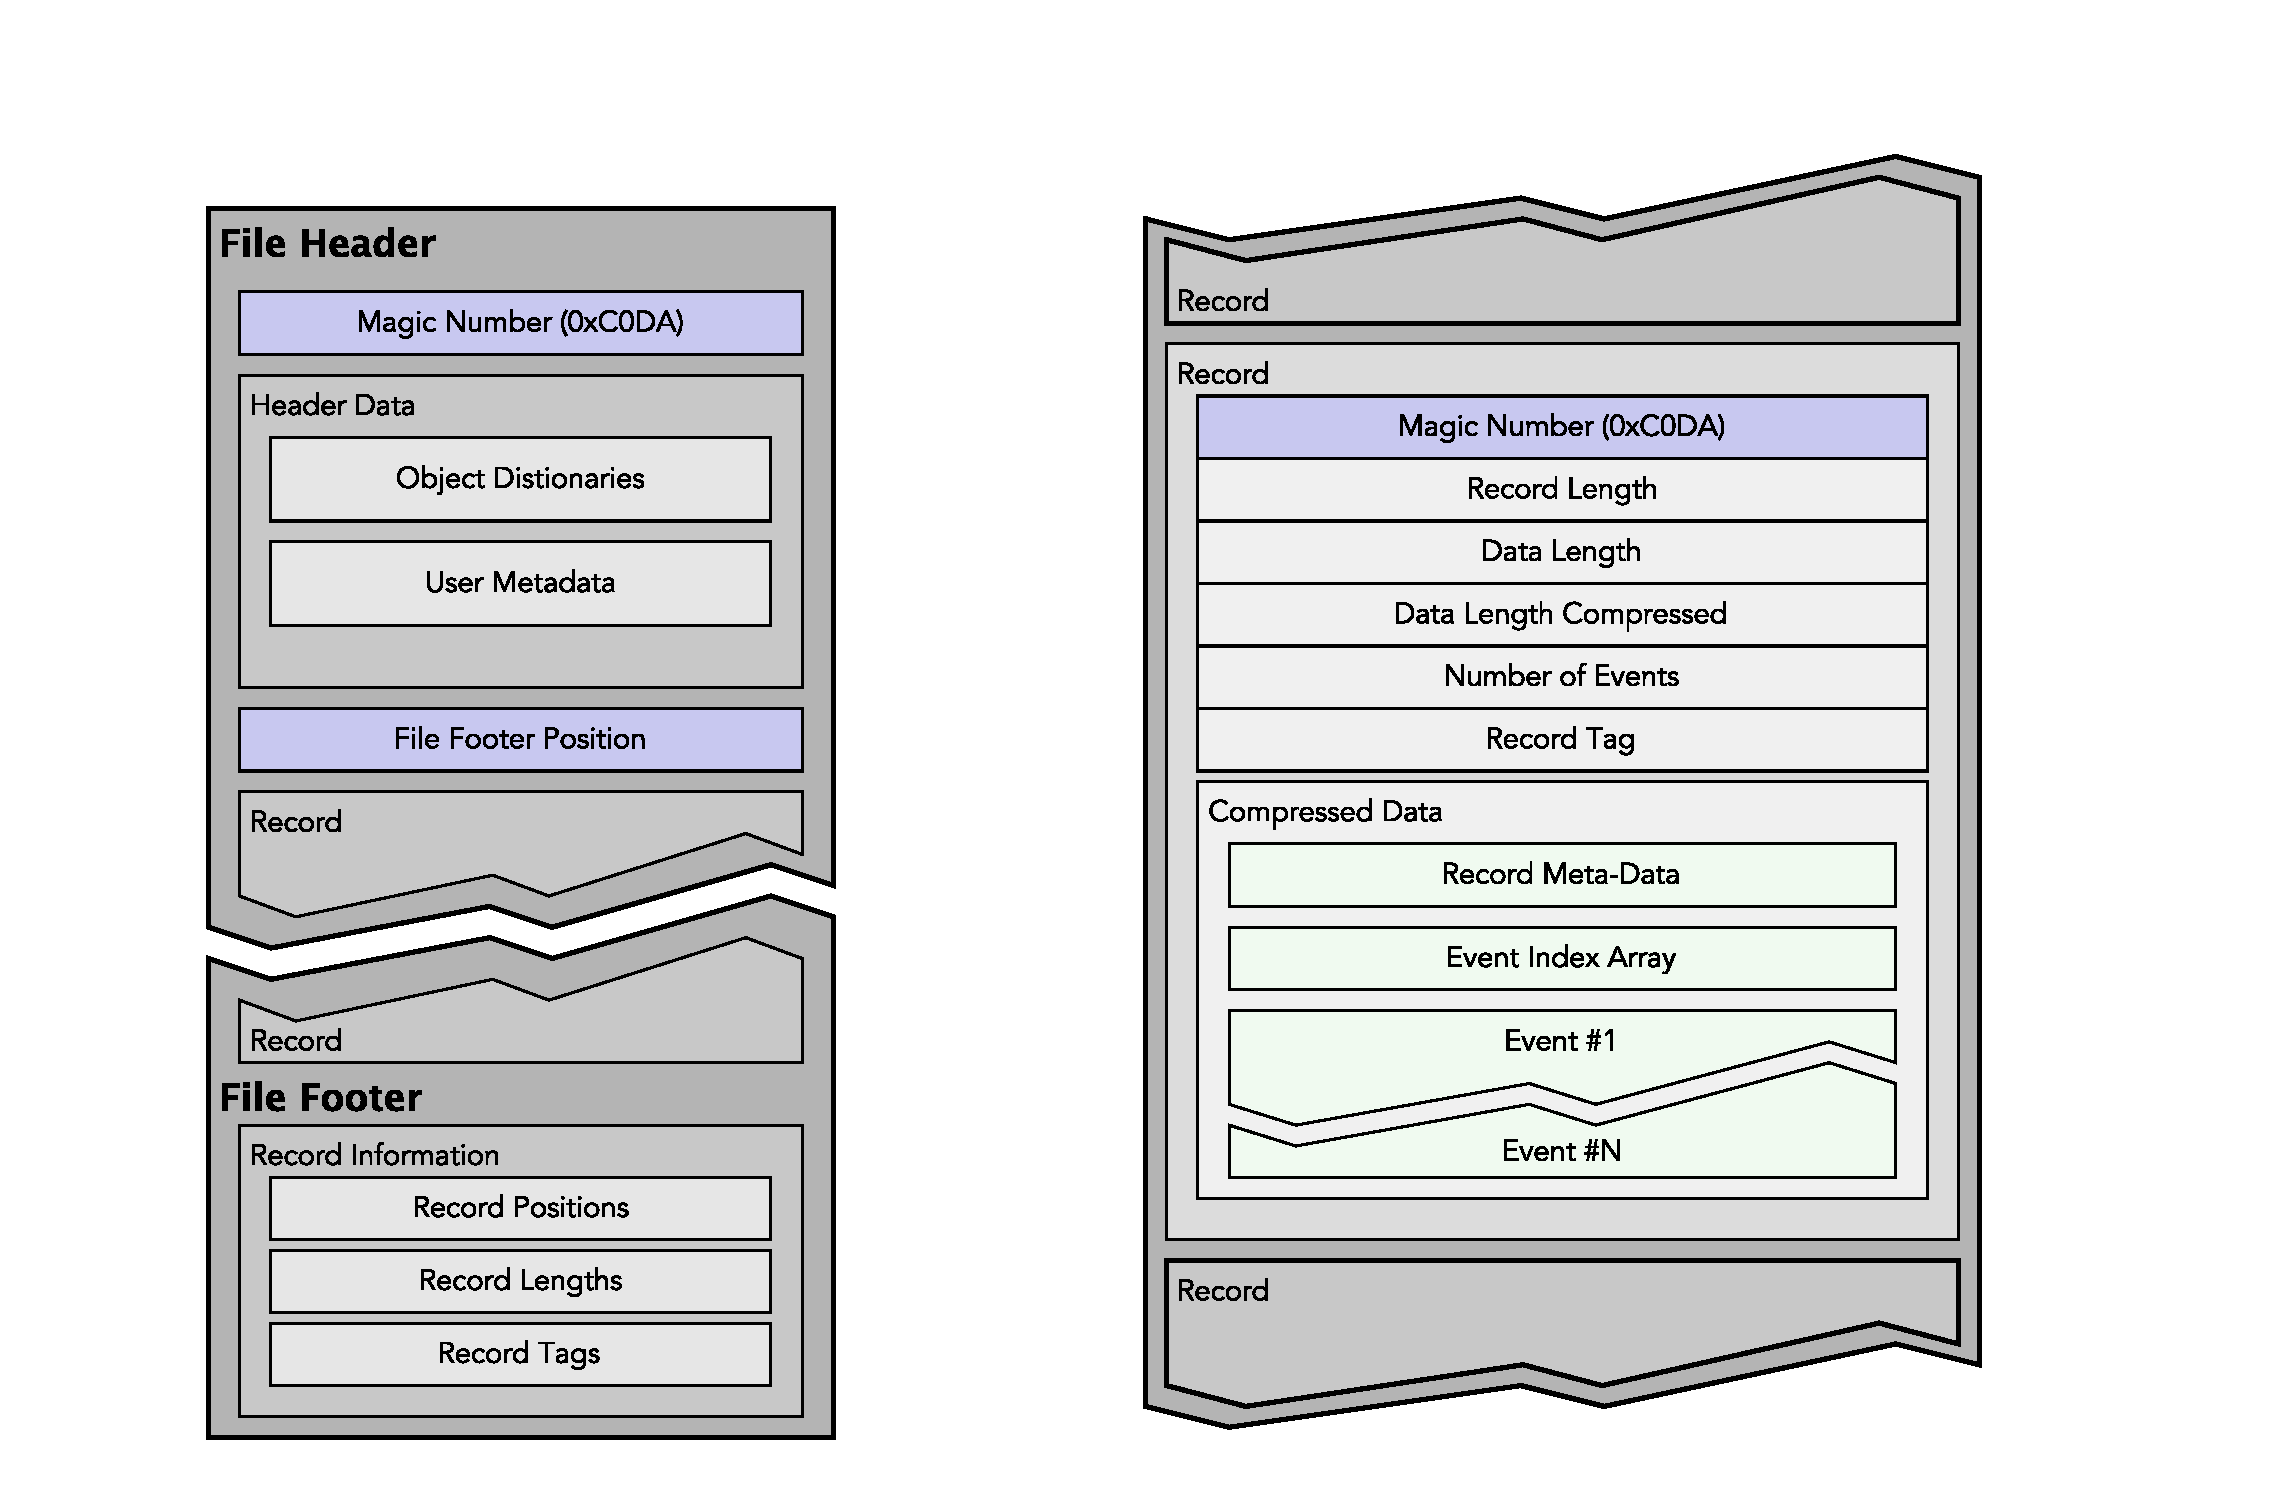
\includegraphics[width=0.85\textwidth]{images/file_structure.pdf}
 \end{center}
  \caption{Schematic view of the HiPO file structure. The figure shows the conceptual design of the file structure. It's not an exact layout of the data structures of the headers. The detailed documentation is published on the GitHub repository with the source code.}
 \label{schema:file}
\end{figure}


\begin{itemize}
\item {\bf File Header:} This section includes essential information such as the file version, file length (used for consistency checks), the location of the file footer, and other relevant parameters.
\item {\bf User Header:} This part contains metadata that describes the content of the file any other user provided metadata. In dictionary-driven formats, it includes descriptors (schemas for tabular data) of the data stored within the file.
\item {\bf Data Records:} These are the compressed, grouped data from individual events. The size of data records is configurable at the time of file creation. Each record is assigned a user-defined identifier, known as a tag, to group similar events together.
\item {\bf File Footer:} The footer contains metadata about each data record in the file, including its position, size, and tag.
The general structure of a HiPO file is illustrated in Figure~\ref{schema:file}.
\end{itemize}

The schematic view of the file structure is shown in Figure~\ref{schema:file}. 

\subsection{File Header}

The file header is a descriptor for the file containing information about the version of the file. This magic word identifies the file format and also carries information about the endianness of the data and the position of the file footer. The header also contains a block of data called "User Data". The user data includes dictionaries of the data objects stored in the file, as well as user-provided metadata describing the file or any parameters the creator may want to include with the file. This metadata comes in the form of key-value pairs usually provided by the user before the file initialization stage. To create a simple file with a given user header, use the code shown in Listing~\ref{lst:open_file}.
%\rule{16.5cm}{0.4pt}
\begin{lstlisting}[language=java, caption=Java example for writing a file with meta-data. The reader object opens the file and retrieves the stored mata data in a form of a key/value map., label=lst:open_file]
// -- open file with user-specified meta data
HipoWriter w = new HipoWriter(); // create the object
w.addConfig("date","created on 01/27/2021");
w.addConfig("author","John Pierce");
w.addConfig("type","Physics Events from A-Detector")
w.open("my_new_file.h5");
w.close();
// -- read metadata from the file
HipoReader r = new HipoReader("my_new_file.h5");
Map<String,String> userInfo = r.getUserConfigurations();
\end{lstlisting}


\subsection{Records}

The records contain data on events stored in sequence. The record header contains information on the number of events stored, an array of indices pointing to each of the events in the buffer, and the length of the data payload before compression and after the compression. The maximum size of the records for each given file is configured at the creation of the file, and the default size is $8~MB$. The record header also contains a unique identifier, which is "0" by default, and events that are added to the file are recorded in sequence in the 
record until the record size limit is reached, at which point the record is compressed and persisted on the disk with the record header attached, and the record is cleared to start receiving the next events. This process continues until the file is closed, at which point the file footer is recorded, containing positions and identifiers of the records. The file header is updated with the position of the file footer for fast access when opening the file for reading.

\subsection{Events}

As it was mentioned above, the HiPO file consists of a series of events. An event is one unit containing a bunch of data objects that are related to each other. The types of data that can be stored in the event are arrays of primitive types and tables. Each object is assigned two identification numbers, which are used to 
retrieve these objects at the read. These identifiers are called "group" (16 bits) and "item" (8 bits). These logical identifiers can be used to group relevant data, use your imagination. The primitive types are simple arrays, and their headers describe the data structure unequivocally and they do not require dictionaries to be read. 

\subsubsection{Primitive types}

The primitive types are arrays of numbers and strings where all elements of the array have the same type (such as byte, short, integer, float, double, long, and string). The objects 
called Node are created from a provided array with user-defined identifiers. The example Listing~\ref{lst:write_arrays} shows how to create their primitive arrays and how to write them into an event:
\rule{16.5cm}{0.4pt}
\begin{lstlisting}[language=java, caption=Java example to create and write primitive types into an event, label=lst:write_arrays]
// Writing arrays into an Event
Event event = new Event(2048); // creta event with max size 2 kB
float[]  df = new float[]{1.0,2.0,3.0,4.0};
short[]  ds = new short[]{3,5,8,13,21,34,55};
Node   nf = new Node(12,1,df);
Node   ns = new Node(12,2,ds);
Node data = new Node(12,3,"Event recorded at 12:52:33"); 
event.write(nf);
event.write(ns);
event.write(data);
\end{lstlisting}

It's worth noting that the preliminary size of the event does not restrict the user to write objects that exceed the allocated event size. As new objects are added to the event, the event buffer 
will adopt the necessary size to accommodate the objects. It is recommended to set the size slightly larger than is needed to avoid reallocations for better performance.

\subsubsection{Tables}

Tables are rectangular data structures with columns and rows. Table objects require a schema (a descriptor) to be able to parse the content. The schema must be created 
and declared before the file is opened for writing since the file writer composes a dictionary and stores all schemas in the header of the file. The data structure that holds
tables is called a Bank and is also assigned two unique identifiers (group, item). The Listing~\ref{lst:write_bank} shows a simple example of how to declare and write a 
simple bank into a file:
\rule{16.5cm}{0.4pt}
\begin{lstlisting}[language=java, caption=Java example to create and write banks (tables) into an event, label=lst:write_bank]
// Writing banks to the event
SchemaBuilder b = new SchemaBuilder("data::clusters",12,1)
    .addEntry("type","B","cluster type") // B - type Byte
    .addEntry("n", "S", "cluster multiplicity") // S - Type Short
    .addEntry("x", "F", "x position") // F - type float
    .addEntry("y","F","y position") // F - type float
    .addEntry("z", "F", "z position"); // F - type Float
// -- create a cchema
  Schema schema = b.build();
// add schema to the file and open the file
  HipoWriter w = new HipoWriter();
  w.getSchemaFactory().addSchema(schema);
  w.addConfig("date","file created at 11:54:22 AM");
  w.addConfig("description","file contains clusters in calorimeter");
  w.open("clusters.h5");                
  Event event = new Event();
  Bank  b  = new Bank(schema,2); // create a table with 2 rows
  b.putByte("type", 0, (byte)   1); b.putByte("type", 1, (byte)   2);
  b.putShort("n"  , 0, (short) 13); b.putShort("n"  , 1, (short) 21);
  b.putFloat("x",0,0.1f); b.putFloat("x",1,0.2f);
  b.putFloat("y",0,1.1f); b.putFloat("y",1,1.2f);
  b.putFloat("z",0,2.1f); b.putFloat("z",1,2.2f);
  event.write(b);
  w.addEvent(event);
  w.close(); // close should be called to write the file footer
\end{lstlisting}

The methods to write and read values for each element in the bank have two interfaces, one using the name of the variable
which makes for more readable code, and the second method using the index of the column which provides better performance 
when needed. The same setters can be used as follows, b.putFloat("x",0,0.1f) $\rightarrow$ b.putFloat(2,0,0.1f), since "x" is the third 
column in the table (column indices are counted starting from "0"). The correct types of setters have to be used when writing the data 
to ensure that the values provided do not overflow the boundaries of the type. However, more generic getters can be used when reading 
the data, such as $getInt(entry, row)$ for all integer types and $getDouble(entry, row)$ for all floating point types.

\rule{15.5cm}{0.4pt}
\begin{lstlisting}[language=java, caption=Java example to read banks from the file, label=lst:read_bank]
HipoReader r = new HipoReader("clusters.h5");        
Bank[] banks = r.getBanks("data::clusters");
// to read more than on bank use: r.getBanks("a","b","c","d");
// If the bank is not present in the event, the returned object 
// will have getRows()==0, no error is generated.
while(r.nextEvent(banks)){
  System.out.printf("\%4d, \%5d, \%8.5f \%8.5f \%8.5f\n",
           banks[0].getInt("type", row),
           banks[0].getInt(1,row),
           banks[0].getFloat("x", row),
           banks[0].getFloat("y", row),
           banks[0].getFloat("z", row));
}
\end{lstlisting}

In Listing~\ref{lst:read_bank} shows how to read the banks from a file and print the content on the screen. The 
$getBanks(String... list)$ method accepts a list of the banks to be read in each event, so multiple banks can be
read and analyzed at once. More advanced examples of how to read events and query the content of the events 
can be found in the examples provided in the repository.

The Listing~\ref{lst:read_bank} provides a simple reading procedure when the banks are automatically read for each event 
for the user. The more complex code can be found in the repository where the Event object is read from the file and then
banks can be read individually from the event, deleted and/or augemented and written into output. 

%\begin{figure}[h!]
%  \begin{center}
%   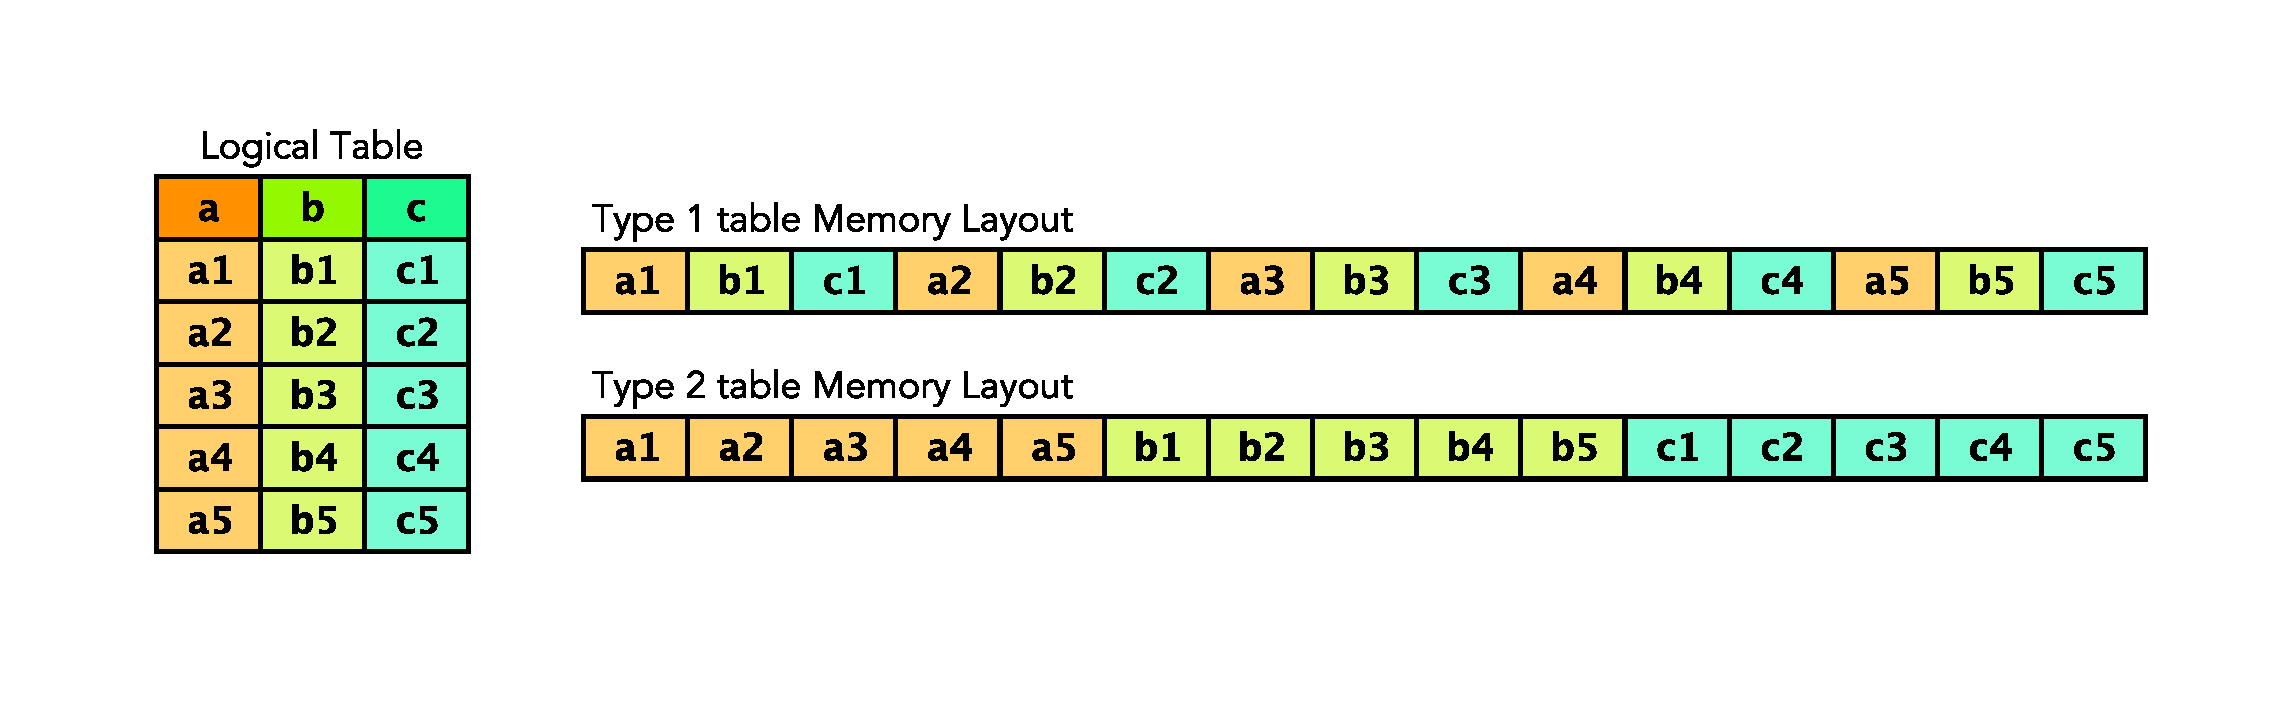
\includegraphics[width=0.95\textwidth]{images/table_layouts.pdf}
% \end{center}
%  \caption{Table types with their memory layout. Type 1 tables are optimized for copying and deleting rows from the table without much overhead on copying individual bytes, while Type 2 tables are better for compression, proving $7\%-15\%$ reduction in the bank size.}
% \label{fig:table_layouts}
%\end{figure}

%The HiPO provides two types of tables where the rows and columns are arranged differently. In the example above
%each column from all the rows is grouped together into a contiguous memory, which makes it necessary to declare 
%the number of rows at the bank creation time and the banks' size can not be changed on the fly. The second type
%is when each row is one contiguous memory block and rows can be altered on the fly, which makes it easy to manipulate
%rows programmatically by removing a row or copying a row into an equivalent table. The schematic view of memory
%mapping for these two types of tables is shown in Figure~\ref{fig:table_layouts}. The reason for having two types of
%tables is that one (the case with columns forming a contiguous memory) is better for data compression which makes
%it more efficient for producing final data sets for analysis. The second table type is used for workflows where different
%components work on the same data set that analyzes the tables by appending and removing entries from a given bank.
%In the particular case of experimental physics usage is the data acquisition system, where a table is growing with incoming
%data, and some rows are removed based on some conditions imposed by the analysis software. In our workflows, the table
%where column values are grouped provides $7\%-15\%$ more compression. Examples of how to use different types of tables
%can be found the the code repository.



%Example usages:
%\begin{verbatim}
%hipo::writer writer("output.file");
%for(int i = 0; i < 12000; i++){
%   hipo::event event = event_provider_next();
%    writer.addEvent(event);
%}
%writer.close();
%\end{verbatim}



%The data from physics experiments is stored in small units called "events", each event contains data related to one physics interaction from a detector. The file consists of a series of events accumulated by the experimental setup during a certain period of time. A HiPO file consists of the following parts:

%- File header: containing file version file length (for consistency check), file footer location, and some other relevant parameters.
%- User header: contains metadata describing the content of the file. In dictionary-driven content contains descriptors of the data 
%stored in the file, the user can add additional information at the creation of the file.
%- Data records: The actual event data grouped and compressed. The size of the data records is configurable at the file creation time. Each record is assigned a user-defined identifier (called tag), which is used to group similar events together.
%- File footer: Contains information about each record in the file, including position, size, and the tag of the record.
%A general structure of the HiPO file is shown in Figure~\ref{hipo_file_structure}.

